\let\negmedspace\undefined
\let\negthickspace\undefined
\documentclass[journal]{IEEEtran}
\usepackage[a5paper, margin=10mm, onecolumn]{geometry}
\usepackage{lmodern} % Ensure lmodern is loaded for pdflatex
\usepackage{tfrupee} % Include tfrupee package

\setlength{\headheight}{1cm} % Set the height of the header box
\setlength{\headsep}{0mm}     % Set the distance between the header box and the top of the text

\usepackage{gvv-book}
\usepackage{gvv}
\usepackage{cite}
\usepackage{amsmath,amssymb,amsfonts,amsthm}
\usepackage{algorithmic}
\usepackage{graphicx}
\usepackage{textcomp}
\usepackage{xcolor}
\usepackage{txfonts}
\usepackage{listings}
\usepackage{enumitem}
\usepackage{mathtools}
\usepackage{gensymb}
\usepackage{comment}
\usepackage[breaklinks=true]{hyperref}
\usepackage{tkz-euclide} 
\usepackage{listings}
\usepackage{gvv}                                        
\def\inputGnumericTable{}                                 
\usepackage[latin1]{inputenc}                                
\usepackage{color}                                            
\usepackage{array}                                            
\usepackage{longtable}                                       
\usepackage{calc}                                             
\usepackage{multirow}                                         
\usepackage{hhline}                                           
\usepackage{ifthen}                                           
\usepackage{lscape}
\begin{document}

\bibliographystyle{IEEEtran}
\vspace{3cm}

\title{9.1.6}
\author{EE24BTECH11005 - Arjun Pavanje}
% \maketitle
% \newpage
% \bigskip
{\let\newpage\relax\maketitle}
\textbf{Question:}
Solve the differential equation $\brak{y^{\prime \prime \prime}}^2 + \brak{y^{\prime \prime}}^3 + \brak{y^{\prime}}^4 + \brak{y}^5 = 0$, with initial conditions $y^{\prime \prime}\brak{x}=0, y^{\prime}\brak{x}=0, y\brak{x}=1$

\solution
An exact theoretical solution using known methods of solving differential equations was not found; however, it can be approximated to a pretty good degree of precision. Euler's method will be used to obtain a plot of the solution\\

Computational Solution:\\
By first principle of derivatives,
\begin{align}
    y^{\prime}\brak{t} = \lim_{h\to 0}\frac{y\brak{t+h} - y\brak{t}}{h}\\
    y\brak{t+h} = y\brak{t} + hy^{\prime}\brak{t}
\end{align}
Let $y^{i}$ be the $i^{th}$ derivative of the function, $m$ be the order of the differential equation. Set $y_1=y, y_2=y^{1}, y_3=y^{2} \dots$ so on.\\
We obtain the system,
\begin{align}
    \myvec{y_1^{\prime} \\ y_2^{\prime} \\ \vdots \\ y_{m-1}^{\prime} }&=\myvec{y_2 \\ y_3 \\ \vdots \\ y_m}\\
y_m^{\prime}&=f\brak{x, y_1, y_2, \dots, y_m}
\end{align}
Generalizing the system according to Euler's form\\
\begin{align}
    \myvec{y_m\brak{x+h} \\ y_{m-1}\brak{x+h} \\ \vdots \\ y_1\brak{x+h}} = \myvec{y_m\brak{x} \\ y_{m-1}\brak{x} \\ \vdots \\ y_1\brak{x}} + h\myvec{f\brak{x, y_1, y_2, \dots, y_m} \\ y_m\brak{x} \\ \vdots \\ y_2\brak{x}}
\end{align}

Discretizing the steps we get,
\begin{align}
    \myvec{\brak{y_{m}}_{n+1} \\ \brak{y_{m-1}}_{n+1} \\ \vdots \\ \brak{y_2}_{n+1} \\ \brak{y_1}_{n+1}}&=\myvec{\brak{y_{m}}_n \\ \brak{y_{m-1}}_n \\ \vdots \\ \brak{y_2}_n \\ \brak{y_1}_n}+h\myvec{f\brak{x, y_1, y_2, \dots, y_m} \\ \brak{y_{m}}_n \\ \vdots \\ \brak{y_3}_n \\ \brak{y_2}_n}\\
    x_{n+1}&=x_n+h
\end{align}
Smaller values of step size $h$ will give more precise plots. We obtain points to plot by iterating repeatedly. 

Given differential equation can be written as,
\begin{align}
    y^{\prime \prime \prime}\brak{x} = \pm \sqrt{-\brak{\brak{y^{\prime \prime}\brak{x}}^3 + \brak{y^{\prime}\brak{x}}^4 + \brak{y\brak{x}}^5 }}
\end{align}
Here, there are two possible functions so we need to take two cases. On substituting given initial conditions we see that we only get valid values for $y^{\prime \prime \prime}\brak{x} = + \sqrt{-\brak{\brak{y^{\prime \prime}}^3 + \brak{y^{\prime}}^4 + \brak{y}^5 }}$. In the other case we observe that we get imaginary values.
\begin{align}
    \myvec{\brak{y_{3}}_{n+1} \\ \brak{y_{2}}_{n+1} \\ \brak{y_1}_{n+1}}=\myvec{\brak{y_{3}}_n \\ \brak{y_2}_n \\ \brak{y_1}_n}+h\myvec{\sqrt{-\brak{\brak{y^{\prime \prime}}^3 + \brak{y^{\prime}}^4 + \brak{y}^5 }}\\ \brak{y_3}_n \\ \brak{y_2}_n}
\end{align}
Below is the plot for given curve  based on initial conditions, obtained by iterating through the above equation.
\begin{figure}[h!]
   \centering
   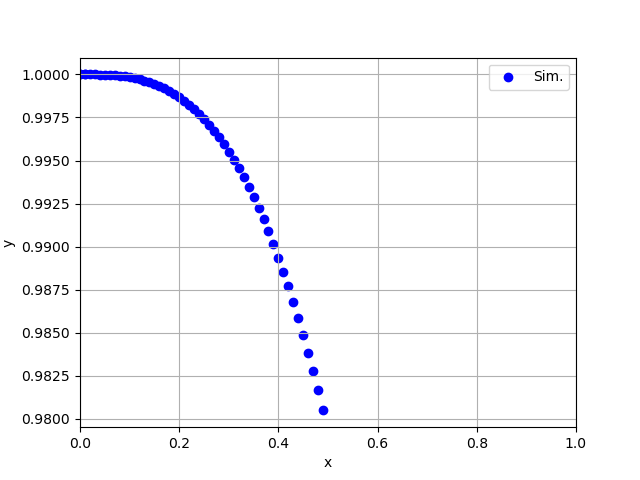
\includegraphics[width=1\columnwidth]{figs/fig1.png}
   \caption{Computational solution of $\brak{y^{\prime \prime \prime}}^2 + \brak{y^{\prime \prime}}^3 + \brak{y^{\prime}}^4 + \brak{y}^5 = 0$}
   \label{stemplot}
\end{figure}

\end{document}

